\documentclass[addpoints, 12pt]{exam}%, answers]
\usepackage[utf8]{inputenc}
\usepackage[T1]{fontenc}

\usepackage{lmodern}
\usepackage{arydshln}
\usepackage[margin=2cm]{geometry}

\usepackage{enumitem}
\usepackage{multicol}

\usepackage{enumerate}
\usepackage{breqn}
\usepackage{parskip}

\usepackage{amsmath, amsthm, amsfonts, amssymb}
\usepackage{graphicx}
\usepackage{tikz}
\usetikzlibrary{arrows,calc,patterns}
\usepackage{pgfplots}
\pgfplotsset{compat=newest}
\usepackage{url}
\usepackage{multicol}
\usepackage{thmtools}

\usepackage{caption}
\usepackage{subcaption}

\usepackage{pifont}

% MATH commands
\newcommand{\bC}{\mathbb{C}}
\newcommand{\bR}{\mathbb{R}}
\newcommand{\bN}{\mathbb{N}}
\newcommand{\bZ}{\mathbb{Z}}
\newcommand{\bT}{\mathbb{T}}
\newcommand{\bD}{\mathbb{D}}

\DeclareMathOperator{\dom}{dom}

\newcommand{\spc}{\vspace*{0.5cm}}
\CorrectChoiceEmphasis{\color{red}}

\begin{document}
\noindent \hrulefill \\
	MATH-241 Calculus I \hfill Created by Rukiyah Walker\\
	Homework 8 \hfill Spring 2023\\ \vspace*{-1cm}
 
	\noindent\hrulefill

\qformat{\rule{0.3\textwidth}{.4pt} \begin{large}{\textsc{Question}} \thequestion \end{large} \hspace*{0.2cm} \hrulefill \hspace*{0.1cm} \textbf{(\totalpoints\hspace*{0.1cm} pts)}}

\begin{questions}

\vspace*{0.5cm}

\question[1]

Let $c$ be a number in the domain $D$ of a function $f(x)$. What is the difference between an absolute maximum and a local maximum?

\begin{choices}
\CorrectChoice The absolute maximum is the largest function value on the entire domain of the function. Whereas the local maximum is the largest function value for some $x$ close to $c$.
\choice They are the same.
\choice The absolute maximum is the largest function value for some $x$ close to $c$. Whereas the local maximum is the largest function value on the entire domain of the function.
\choice An absolute maximum is the value of $f$ when $f(x) \geq f(c)$ for some $x$ close to $c$. The local maximum is the value of $f$ when $f(c) \geq f(x)$ for all $x$ in the entire domain.
\end{choices}

\question[1]


Use the graph to identify the absolute and local maximum and minimum values of the function.

\begin{minipage}{0.5\textwidth}
\begin{choices}
\choice Absolute maximum at 5, absolute minimum at 2. Local maximum at 3, local minimum at 4.\vspace*{10pt}
\choice Absolute maximum at 3, absolute minimum at 1. Local maximum at 2, local minimum at 0.5 and at 1.\vspace*{10pt}
\CorrectChoice Absolute maximum at 5, absolute minimum at 2. Local maximum at 3, local minimum at 2 and at 4.\vspace*{10pt}
\choice Absolute maximum at 3, absolute minimum at 1. Local maximum at 2, local minimum at 1.\vspace*{10pt}
\end{choices}
\end{minipage}
\hspace*{1cm}
\begin{minipage}{0.35\textwidth}
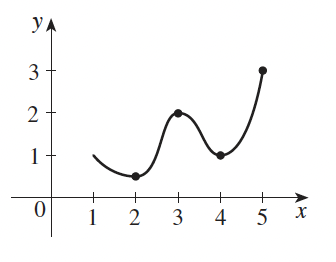
\includegraphics[width=1\textwidth]{HW4-graph.png}
\end{minipage}

\question[1]

We use the Extreme Value Theorem to:

\begin{choices}
\choice Show that a function is continuous on a closed interval $[a, b]$. 
\choice Prove the existence of local maximum and minimum values of a continuous function on a closed interval $[a, b]$.
\choice To show that a function exists on a closed interval $[a, b]$.
\CorrectChoice Prove the existence of absolute maximum and minimum values of a continuous function on a closed interval $[a, b]$.
\end{choices}

\question[1]

What does Fermat's Theorem mean in terms of critical numbers?

\begin{choices}
\choice For some critical number $c$, in the domain of $f$, $f'(c)$ does not exist.
\choice If $f'(c)$ exists and $f'(c) = 0$, then $f$ has a local maximum or minimum at $c$.
\CorrectChoice If $f$ has a local maximum or minimum at $c$, then $c$ is a critical number of $f$.
\choice If $f$ has a local maximum or minimum at $c$, then $f'(c)$ does not exist.
\end{choices}

\spc

\question[1]

We use Rolle's Theorem to:

\begin{choices}
\choice Show that the derivative of a function exists.
\CorrectChoice Show that the graph of a function has a horizontal tangent line. 
\choice Show that there exists a continuous function. 
\choice If $f$ has a local maximum or minimum at $c$, then $f'(c)$ does not exist.
\end{choices}

\spc

\question[1]

We use the Mean Value Theorem to:

\begin{choices}
\CorrectChoice Show that there is at least one point, on the graph of a function, where the slope of the tangent line is the same as the slope of the secant line.
\choice Show that the derivative of a function exists.
\choice Show that a function $f$ is continuous on the closed interval $[a, b]$.
\choice Show that the graph of a function has a horizontal tangent line. 
\end{choices}

\question[1]

f(x) = $\frac{1}{x}$. Find the number $c$ that satisfies the conclusion of the Mean Value Theorem on the interval [1, 3].

\begin{multicols}{2}
\begin{choices}
\choice $c = \pm\sqrt{\frac{3}{2}}$
\CorrectChoice $c = \sqrt{3}$
\choice $c = \sqrt{\frac{2}{3}}$
\choice $c = \pm\sqrt{3}$
\end{choices}
\end{multicols}


\question[1]

When will a function $f$ be a constant function?

\begin{choices}
\choice When $f'(x)$ does not exist. 
\choice When $f(x)$ is continuous.
\choice When $f(x)$ is everywhere differentiable.
\CorrectChoice When $f'(x) = 0$.
\end{choices}

\spc

\question[1]

Suppose that $c$ is a critical number of a continuous function $f$.
Fill in the blank: 

If $f'$ changes sign from positive to negative at c, then ____. 
\newline If $f'$ changes sign from negative to positive at c, then ____.

\begin{multicols}{2}
\begin{choices}
\choice $f$ has no local maximum.

$f$ has no local minimum.
\CorrectChoice $f$ has a local maximum at $c$.

$f$ has a local minimum at $c$.
\choice $f$ has an absolute maximum at $c$.

$f$ has an absolute minimum at $c$.
\choice $f$ has a local minimum at $c$.

$f$ has a local maximum at $c$.

\end{choices}
\end{multicols}



\question[1]

Use the graph to identify the local maximum and minimum values of the function.\vspace*{10pt} 

\begin{minipage}{0.5\textwidth}\vspace*{2pt}
\begin{choices}
\choice Local minimum at $x = 3$. No Local maximum.\vspace*{10pt}
\choice Local minimum and maximum at $x = 3$.\vspace*{10pt}
\CorrectChoice No local maximum or minimum.\vspace*{10pt}
\choice No local minimum, local maximum at $x = 3$.\vspace*{10pt}
\end{choices}
\end{minipage}
\hspace*{1cm}
\begin{minipage}{0.45\textwidth}
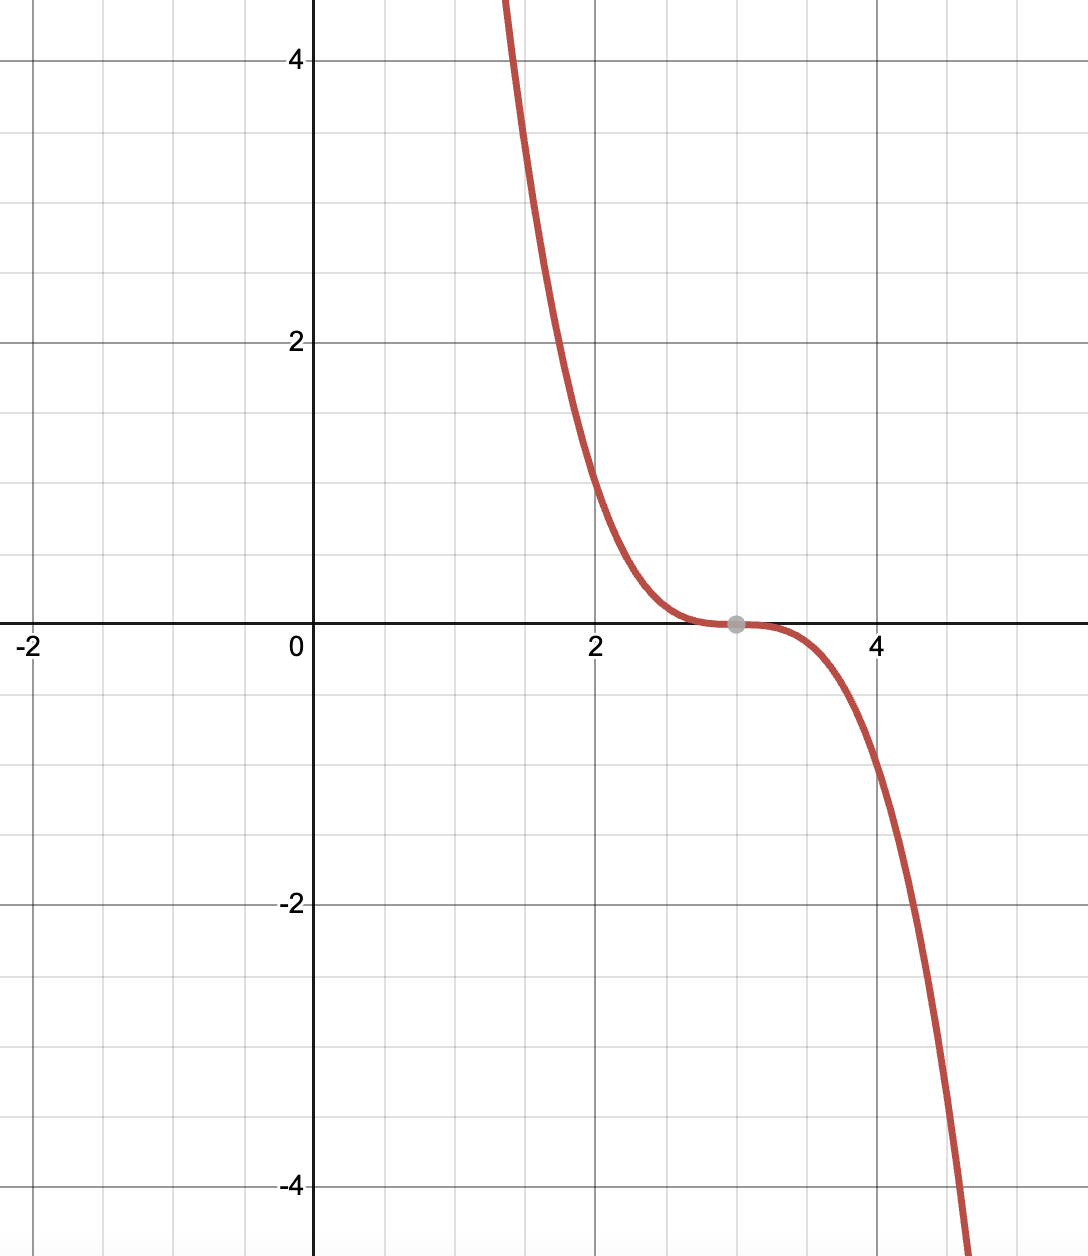
\includegraphics[width=0.75\textwidth]{HW4-graph1.png}
\end{minipage}


\end{questions}
\end{document}